% This is samplepaper.tex, a sample chapter demonstrating the
% LLNCS macro package for Springer Computer Science proceedings;
% Version 2.20 of 2017/10/04
%
\documentclass[runningheads]{llncs}
%
\usepackage{graphicx}
\usepackage{csquotes}
\usepackage{hyperref}
% Used for displaying a sample figure. If possible, figure files should
% be included in EPS format.
%
% If you use the hyperref package, please uncomment the following line
% to display URLs in blue roman font according to Springer's eBook style:
% \renewcommand\UrlFont{\color{blue}\rmfamily}

\begin{document}
%
\title{Evolution of the Spineless Tagless G-Machine}
%
%\titlerunning{Spineless Tagless G-Machine}
% If the paper title is too long for the running head, you can set
% an abbreviated paper title here
%
\author{Armin Bernstetter}
%
\authorrunning{Armin Bernstetter}
% First names are abbreviated in the running head.
% If there are more than two authors, 'et al.' is used.
%
\institute{Seminar Funktionale Programmierung \\ Julius-Maximilians-Universität, Würzburg}
%\institute{Princeton University, Princeton NJ 08544, USA \and
%Springer Heidelberg, Tiergartenstr. 17, 69121 Heidelberg, Germany
%\email{lncs@springer.com}\\
%\url{http://www.springer.com/gp/computer-science/lncs} \and
%ABC Institute, Rupert-Karls-University Heidelberg, Heidelberg, Germany\\
%\email{\{abc,lncs\}@uni-heidelberg.de}}
%
\maketitle              % typeset the header of the contribution
%
\begin{abstract}
The spineless tagless G-machine (STGM) is an abstract machine that is located at the core of the Glasgow Haskell Compiler GHC. Since its creation at the start of Haskell development in early 1990s it has undergone several significant changes. This work aims at showing the evolution of the STGM and overall at providing insight in the workings of the most widely-used Haskell compiler GHC.

%\keywords{First keyword  \and Second keyword \and Another keyword.}
\end{abstract}
%
%
%

\section{Introduction}

This work provides an insight in the compilation process of the lazy, pure functional programming language Haskell. For this we take a look inside the Glasgow Haskell Compiler, today the most used compiler for Haskell [citation needed]. Located at its core is the \textit{Spineless Tagless G-Machine}, an abstract machine used as a bridge between high level code and machine code.

Described in detail in the 1992 paper \textit{Implementing Lazy functional languages on stock hardware: the Spineless Tagless G-machine} \cite{jones1992implementing}, the STGM has undergone several significant changes since then. Two papers highlighting these changes are \textit{Making a Fast Curry: Push/Enter vs.
Eval/Apply for Higher-order Languages}\cite{marlow2004making} and \textit{Faster Laziness Using Dynamic Pointer Tagging}\cite{marlow2007faster}. The former introducing the switch from the \textit{push/enter} evaluation method to the \textit{eval/apply} (see section BLA), the latter introducing dynamic pointer tagging which revokes the \enquote{tagless} part in the name of the STGM.

Section \ref{sec:basics} provides basic information about Haskell and compilers in general.

Section \ref{sec:ghc} describes GHC, the \textit{Glasgow Haskell Compiler} which is the most widely-used Haskell compiler. This section introduces the building blocks that GHC consists of.

Section \ref{sec:stgm} takes a more in-depth look into the \textit{Spineless Tagless G-Machine}, an abstract machine that stands between Haskell code and assembly code in GHC's compilation process.

Section \ref{sec:conclusion} concludes with a retrospective overview of STGM and its changes throughout the last 30 years.



\section{Basics}
\label{sec:basics}

This section introduces basics about compilers, Haskell and functional programming in general.

\subsection{Haskell}
Haskell is a pure functional programming language that emerged during the late 1980s and early 1990s. It was created with the goal of finding a common functional language to improve interactivity and exchange between programmers and researchers since, at the time, many lesser known functional programming languages existed. A committee consisting of Paul Hudak, John Hughes, Simon Peyton Jones, Philip Wadler and others was created and met several times until in 1990 the Haskell 1.0 Report was published \cite{hudak2007history}.

\subsection{Compilers}
A compiler is a software system consisting of several phases, that translates programs from a higher-level language to machine code. \cite{muchnick1997advanced}

In general, these phases are \textit{lexical analysis}, \textit{syntactic analysis or parsing}, \textit{semantic checking} and \textit{code generation}. \cite{muchnick1997advanced}

\paragraph{Lexical Analysis} analyzes the character string and produces errors in case any part of the program string is not parseable into legal tokens. Legal in this case refers to tokens that are members of the vocabulary of the respective programming language.

\paragraph{Syntactic Analysis or Parsing} parses the program into an intermediate representation. An example would be a parse tree accompanied by a symbol table containing information on identifiers used in the program and their attributes. This phase may also produce error messages if syntax errors are detected.

\paragraph{Semantic Checking} examines the program for static-semantic validity. This phase takes as input the intermediate representation and determines whether the program satisfies the requirements for the static-semantic properties of the source language.

\paragraph{Code Generation} finally transforms the intermediate representation into machine code which can then be executed. 


These phases are often complemented by additional steps in many compilers, the Glasgow Haskell Compiler being one of those (see Section \ref{sec:ghc}).

\subsection{Abstract machines}
What is an Abstract machine?
\cite{diehl2000abstract}

\section{GHC}
\label{sec:ghc}

\href{https://downloads.haskell.org/~ghc/7.8.1/docs/html/users_guide/an-external-representation-for-the-ghc-core-language-for-ghc-6.10.html}{link ghc 7.8.1}

\href{https://downloads.haskell.org/ghc/8.6.5/docs/html/users_guide}{link ghc 8.6.5}

The Glasgow Haskell Compiler, named after the city where its development was initialized, is the most widely-used Haskell compiler \cite{marlow2007faster}.



\subsection{Core Language}
The core language is a variant of Haskell in where all syntactic sugar is removed and resolved e.g. the do-notation or type aliases. It consists of GHC's central data types and is a small, explicitly-typed variant of System F \cite{girard1986system} which is called System FC \cite{sulzmann2007system}.


\subsection{The STGM Language}
The STG language is a pure functional programming language on its own. Reduced to the very basics it directly interacts with the stack and heap through the STG machine.[citation needed]

syntax details?

heap object layouts?


\subsection{$C--$}
$C - - $ is a language developed by Simon Peyton-Jones as a portable backend-language for compilers. Its name references C and C++. Where C++ can be seen as an extension of the C language, C-- is to be thought of as a reduction to a smaller core language. C-- in general is made for being generated by compilers and not for being written by programmers.

\paragraph{Why is it needed? C and Stack stuff?}


\subsection{Backends}
GHC supports the generation of Assembly machine code via several backends.


\subsubsection{C Backend}
The C backend uses GCC but is deprecated

\subsubsection{Native Code Generator}
The Native Code Generator is the default way used in GHC.

\subsubsection{LLVM}
LLVM is a modern portable compiler toolchain that was developed as an alternative to the classic GCC toolchain. \cite{lattner2004llvm}

Using LLVM in GHC results in similar compilation performance as the NCG but can lead to faster performing executables.

\section{STGM in depth}
\cite{jones1992implementing}
\label{sec:stgm}

\subsubsection{Spineless}
Spineless refers to the way the code is represented on the machine.

STG programs are not represented as a tree but as a graph. Therefore, in memory a STG program is not a contiguous block of memory but smaller parts of the graph that reference each other.

\subsubsection{Tagless}
The term tagless refers to the way the STG-machine evaluates a heap closure. 


[EVERYTHING FROM THE INTRODUCTION OF THE POINTER TAGGING PAPER]


\subsection{Evaluation/function calls}
Function calls in a lazy functional languages with currying and partial application require special mechanisms in compilers.
\enquote{Currying} is one of the core principles of lazy functional languages 

[INSERT DETAILS ABOUT CURRYING]


HOW TO INCLUDE THE EVALUATION TRACE?



\subsubsection{Push/Enter}
\subsubsection{Eval/Apply}

\subsection{Dynamic Pointer Tagging}
In 2007, Marlow et al.\cite{marlow2007faster} found, that Haskell programs compiled by GHC show mispredicted branches on modern processors. This led to a re-examination of the \enquote{tagless} aspect of the GHC. The result were significant performance improvements.


\section{Conclusion}
\label{sec:conclusion}


\section{First Section}
\subsection{A Subsection Sample}
Please note that the first paragraph of a section or subsection is
not indented. The first paragraph that follows a table, figure,
equation etc. does not need an indent, either.

Subsequent paragraphs, however, are indented.

\subsubsection{Sample Heading (Third Level)} Only two levels of
headings should be numbered. Lower level headings remain unnumbered;
they are formatted as run-in headings.

\paragraph{Sample Heading (Fourth Level)}
The contribution should contain no more than four levels of
headings. Table~\ref{tab1} gives a summary of all heading levels.

\begin{table}
\caption{Table captions should be placed above the
tables.}\label{tab1}
\begin{tabular}{|l|l|l|}
\hline
Heading level &  Example & Font size and style\\
\hline
Title (centered) &  {\Large\bfseries Lecture Notes} & 14 point, bold\\
1st-level heading &  {\large\bfseries 1 Introduction} & 12 point, bold\\
2nd-level heading & {\bfseries 2.1 Printing Area} & 10 point, bold\\
3rd-level heading & {\bfseries Run-in Heading in Bold.} Text follows & 10 point, bold\\
4th-level heading & {\itshape Lowest Level Heading.} Text follows & 10 point, italic\\
\hline
\end{tabular}
\end{table}


\noindent Displayed equations are centered and set on a separate
line.
\begin{equation}
x + y = z
\end{equation}
Please try to avoid rasterized images for line-art diagrams and
schemas. Whenever possible, use vector graphics instead (see
Fig.~\ref{fig1}).

\begin{figure}
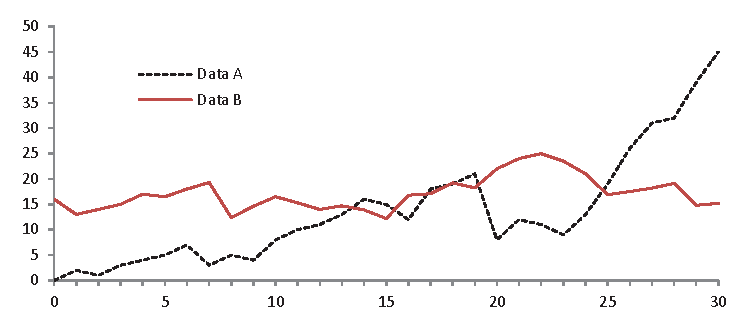
\includegraphics[width=\textwidth]{fig1.eps}
\caption{A figure caption is always placed below the illustration.
Please note that short captions are centered, while long ones are
justified by the macro package automatically.} \label{fig1}
\end{figure}

\begin{theorem}
This is a sample theorem. The run-in heading is set in bold, while
the following text appears in italics. Definitions, lemmas,
propositions, and corollaries are styled the same way.
\end{theorem}
%
% the environments 'definition', 'lemma', 'proposition', 'corollary',
% 'remark', and 'example' are defined in the LLNCS documentclass as well.
%
\begin{proof}
Proofs, examples, and remarks have the initial word in italics,
while the following text appears in normal font.
\end{proof}
For citations of references, we prefer the use of square brackets
and consecutive numbers. Citations using labels or the author/year
convention are also acceptable. The following bibliography provides
a sample reference list with entries for journal
articles~\cite{ref_article1}, an LNCS chapter~\cite{ref_lncs1}, a
book~\cite{ref_book1}, proceedings without editors~\cite{ref_proc1},
and a homepage~\cite{ref_url1}. Multiple citations are grouped
\cite{ref_article1,ref_lncs1,ref_book1},
\cite{ref_article1,ref_book1,ref_proc1,ref_url1}.
%
% ---- Bibliography ----
%
% BibTeX users should specify bibliography style 'splncs04'.
% References will then be sorted and formatted in the correct style.
%
\bibliographystyle{splncs04}
\bibliography{stgm.bib}
%
%\begin{thebibliography}{8}
%\bibitem{ref_article1}
%Author, F.: Article title. Journal \textbf{2}(5), 99--110 (2016)
%
%\bibitem{ref_lncs1}
%Author, F., Author, S.: Title of a proceedings paper. In: Editor,
%F., Editor, S. (eds.) CONFERENCE 2016, LNCS, vol. 9999, pp. 1--13.
%Springer, Heidelberg (2016). \doi{10.10007/1234567890}
%
%\bibitem{ref_book1}
%Author, F., Author, S., Author, T.: Book title. 2nd edn. Publisher,
%Location (1999)
%
%\bibitem{ref_proc1}
%Author, A.-B.: Contribution title. In: 9th International Proceedings
%on Proceedings, pp. 1--2. Publisher, Location (2010)
%
%\bibitem{ref_url1}
%LNCS Homepage, \url{http://www.springer.com/lncs}. Last accessed 4
%Oct 2017
%\end{thebibliography}
\end{document}
